\subsubsection{Computational Systems Biology}
\index{H\"utt, Marc-Thorsten}

\paragraph{Research Team}
%
Marc-Thorsten H\"utt (Professor), Manuel Dehnert (Postdoc), Daniel Geberth (PhD Student), Carsten Marr (PhD Student), Mark M\"uller-Linow (PhD Student), Heike Hameister (Graduate Student), Niko Sonnenschein (Graduate Student) \\

Research of the Computational Systems Biology group focuses on three key topics: biological networks, genome evolution and pattern formation. In essence, we want to understand:
\begin{myitemize}
\item which patterns in gene expression data are related to topological features of the underlying transcriptional regulatory networks;

\item how metabolic fluxes are organized and how patterns of flux redistribution under perturbations come about;

\item how the networks of gene regulation, protein interactions and metabolism interact to organize cellular function;

\item how (statistical) patterns in genome-wide DNA sequences correspond to (or are a consequence of) specific processes of genome evolution;

\item how a measured pattern of cell-cell differences may help predict the precise layout of spatiotemporal structures in \textit{Dictyostelium} self-organization.

\end{myitemize}

In previous years we have particularly established the following methods:

\textit{Biological networks} We have designed a one-parameter class of cellular automata, which can be implemented on arbitrary graphs. With this model system we can quantify the pattern formation capacity of synthetic and real networks.

\textit{Genome evolution} We have shown that patterns in the short-range statistical correlations in DNA sequences serve as an eukaryotic genome signature.  All chromosomes of a species display the same characteristic pattern, markedly different from those of other species.

\textit{Pattern formation} We have shown that in chains of coupled nonlinear oscillators biological variability can induce complex spatiotemporal pattern.


\paragraph{Highlights}
%
The group has moved to IUB in May 2006. It was previously located at
Darmstadt University of Technology. \newline\newline On the level of
research we have achieved the following results in 2006:

\textit{Biological networks} Despite their topological complexity almost all functional properties of metabolic networks can
be derived from steady-state dynamics. Indeed, many theoretical investigations (like flux-balance
analysis) rely on extracting function from steady states. This leads to the interesting question, how
metabolic networks avoid complex dynamics and maintain a steady-state behavior. We exposed
metabolic network topologies to binary dynamics generated by simple local rules. We find that the
network's response is highly specific: Complex dynamics are systematically reduced on metabolic
network topologies compared to networks with similar topologies. Already small topological modifications
substantially enhance the capacity of a network to host complex dynamic behavior and
thus reduce its regularizing potential. This exceptionally pronounced regularization of dynamics
encoded in the topology may explain, why steady-state behavior is ubiquitous in metabolism \cite{MarrEtAl2006}.

We also studied the average excitation density in a simple model of excitable dynamics on graphs and find that this
density is changed
via the distribution pattern of excitations: An increase in connectivity induces a transition from globally to
locally organized excitations and, as a result, leads to an increase in the excitation density. A similar transition
can be induced by increasing the rate of spontaneous excitations while keeping the graph architecture constant \cite{MuellerLinowEtAl2006}.

Furthermore, we looked at the effect of shortcuts on dynamics in regular graphs. It is known that shortcuts in a regular architecture affect the information transport through the system due to the severe decrease in average path length. Our fundamentalnew perspective in terms of pattern formation is the destabilizing effect of topological perturbations by processing distant uncorrelatedinformation, similarly to stochastic noise. We studied this functional coincidence of rewiring and noisy communication on patterns of binary cellular automata \cite{MarrHuett2006}.


\textit{Genome evolution} For the examples of \textit{Mus musculus}
and \textit{Rattus norvegicus} we analyzed in detail short- and intermediate-range statistical correlations in DNA sequences.
These correlation profiles have been computed for all chromosomes of the two species. We find that with increasing
range of correlations the capacity to distinguish between the species on the basis of this correlation profile is
getting better and requires ever shorter sequence segments for obtaining a full species separation. This finding for the first time suggests that distinctive traits within the sequence are situated beyond the level of few nucleotides \cite{DehnertEtAl2006}.

\textit{Pattern formation} This project was started in 2006 and already shows very promising results. We are currently comparing a variety of statistical methods to extract systematic cell-to-cell differences in the case of patterns formed by the slime mould \textit{Dictyostelium discoideum}. We discuss, to what extent these cell properties can serve as predictors of certain later-stage patterns. This work is carried out together with the group of S.C. M�ller (Magdeburg). On the level of modeling, we are investigating how an initial distribution of pacemaker cells is translated by the process of self-organization into a pattern of fully developed spiral waves, represented by a distribution of phase singularities.

On the level of teaching and scientific communication, this year's clear and distinct highlight  for us was to see our new Bioinformatics textbook published by Springer-Verlag \cite{HuettDehnert2006}. Furthermore, a new edited volume on interdisciplinary aspects of self-organization has been published by B\"ohlau-Verlag \cite{VecEtAl2006}. The two-week visit by Professor Larry S. Liebovitch at Jacobs University within the ICTS program in October has helped us reach a new level in our collaboration and write and submit a manuscript summarizing our previous work.


\begin{figure}[ht]
  \begin{center}
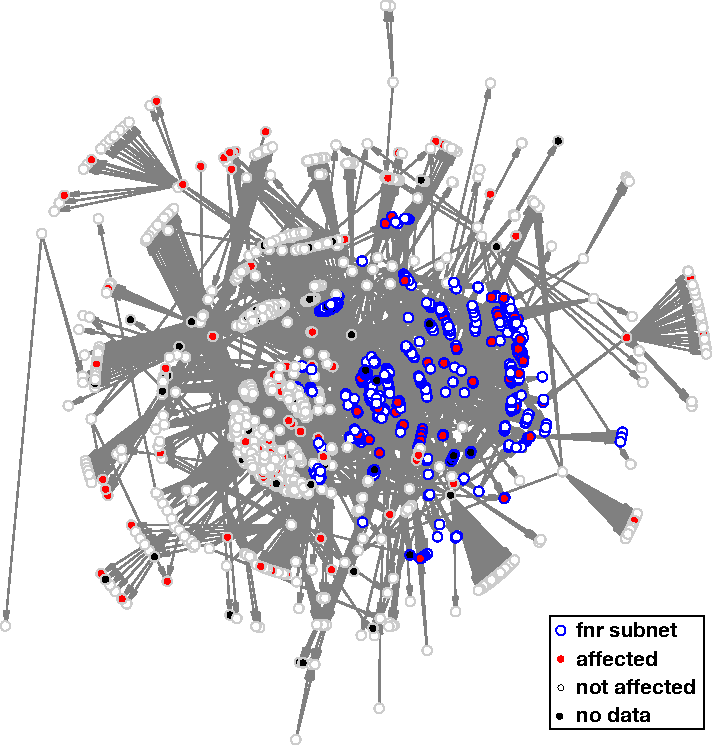
\includegraphics[width=\hsize]{Huett/huett_fig1.pdf}
    \mycaption{ Effect of fnr deletion under anaerobic growth conditions in the largest connected component of the transcriptional regulatory network of \textit{E. coli}. All genes downstream fnr are labeled by a blue circle. We count genes as affected (red disc), when expression levels of wildtype and mutant differ significantly (p value $<$ 0.05). Apparently, the mutation affects many nodes beyond the fnr subnet, indicating that the network compensates for the loss of fnr collectively.}\label{fig:profHuett}
   \end{center}
\end{figure}

\paragraph{Organization}
%
\begin{enumerate}
\item Chair and member of the organizing committee of the British-German Frontiers of Science Meeting 2006 (jointly organized by the Royal Society and the Alexander von Humboldt Foundation)
\item Elected into the Editorial Board of Nonlinear Biomedical Physics (NBP)
\end{enumerate}

\myparagraph{Collaborations}
%
Bremen Area Collaborations:
\begin{enumerate}
\item {\sl International University Bremen} \\ Prof. F.O. Gl�ckner  \\ Genome signatures
 \\Prof. H. Meyer-Ortmanns \\ Discrete and continuous formulations
of excitable dynamics on graphs  \\ Prof. G. Muskhelishvili \\ A
network view on \textit{E. coli} gene expression  \\ Prof. M.
Zacharias \\Topology of protein interaction networks
\end{enumerate}
National \& International Collaborations:
\begin{enumerate}
\item {\sl Florida Atlantic University} \\  Prof. L.S. Liebovitch \\ Transcriptional regulatory network properties in gene expression profiles
\item {\sl Darmstadt University of Applied Sciences} \\  Prof. W.E. Helm \\ Statistical correlations in DNA sequences
\item {\sl Darmstadt University of Technology} \\  Prof. M. Porto \\ Reaction-diffusion processes on scale-free networks
\item {\sl Darmstadt University of Technology} \\ Prof. C. Weihe, Dr. M. M\"uller-Hannemann \\ Impact of motif content on dynamic function of complex networks
\item {\sl Magdeburg University} \\ Prof. S.C. M�ller \\ \textit{Dictyostelium} pattern formation
\item {\sl Max Planck Institute of Molecular Plant Physiology} \\  Dr. W. Weckwerth \\ Consistency of metabolic correlation networks with genome-derived pathway structures
\end{enumerate}


\paragraph{Grants}
\begin{enumerate}
\item Funded by DFG,  \emph{Role of biological variability in the
pattern formation of \textit{Dictyostelium discoideum}, HU-937/4},
(May 2006 - April 2009)
\end{enumerate}

\newpage
\paragraph{Awards, Prizes}
\begin{enumerate}
\item W.E. Heraeus summer school on {\it Statistical Physics of
Gene Regulation: From Genetic Networks to Expression Data and Back
} (organized with H. Meyer-Ortmanns) to take place in July 2007, approved in 2006
\end{enumerate}

\nocite{MarrEtAl2006}
